%
% fig-sl.tex
%
% (c) 2025 Prof Dr Andreas Müller
%
\begin{figure}
\centering
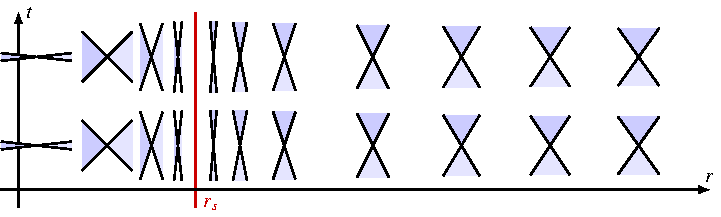
\includegraphics{chapters/110-kruemmung/images/sl.pdf}
\caption{Entstehung des Ereignishorizontes bei einem schwarzen Loch.
Ausserhalb von $r=r_s$ zeigen
die Vektoren mit negativem Minkowski-Metrik (zeitartige Vektoren)
in Richtung Zukunft (blau) oder Vergangenheit (hellblau).
Innerhalb $r=r_s$ ist die Richtung der Zukunft ausschliesslich zu
abnehmenden Werten von $r$ gerichtet.
Teilchen können sich also nur noch auf Bahnen bewegen, die innerhalb
$r_s$ bleiben.
\label{buch:kruemmung:schwarzesloch:fig:sl}}
\end{figure}

